\begin{song}{title=\predtitle\centering Pohádka \\\large Karel Plíhal\vspace*{-0.5cm}}  %% sem se napíše jméno songu a autor
\begin{centerjustified}
\mezera \noindent \textbf{Rec:}
Takhle nějak to bylo: jedlo se, zpívalo, pilo,

princezna zářila štěstím v hotelu nad náměstím,

drak hlídal u dveří sálu, na krku pletenou šálu,

Dědové Vševědi okolo Popelky žvatlavě slibují šaty a kabelky,

každý si odnáší kousíček úsměvu,

dešťový mraky se chystaly ke zpěvu,

hosté se sjíždějí k veliké veselce,

paprsky luceren metají kozelce

a stíny ořechů orvaných dohola

pletou se latícím kočárům pod kola,

Šmudla si přivezl v odřeným wartburgu

kámošku z dětství, prej nějakou Sněhurku,

vrátný se zohýbá pro tučné spropitné

a kdo mu proklouzne, tak toho nechytne,

kouzelník za dvacku vykouzlí pět bonů

a vítr na věži opřel se do zvonů,

„Na zdraví nevěsty, na zdraví ženicha!“,

dvě sousta do kapsy a jednou do břicha,

náhle se za oknem objevil skřítek,

rozhrnul oponu z máminejch kytek,

pěkně se usmál a pěkně se podíval

a pak mi po očku do ucha zazpíval:


\refren
^{G\,\,}Dej mi ruku ^{D{\z}}svou, ^{{\z}Emi}studenou od okenních ^{Hmi/D}skel,

všichni tě ^{C{\z}}mezi sebe ^{Hmi/D}zvou

a ^{C}já jsem ^{D}tu proto, ^{G{\z}}abys ^{{\z}Emi}šel.~


\mezera \noindent \textbf{Rec:}
Na plný obrátky letíme světem,

všechny ty pohádky patřily dětem,

dneska už se neplatí buchtama za skutky,

sudičky sesmolí kádrový posudky,

obložen prošlými dlužními úpisy,

koukám se z okna a vzpomínám na kdysi,

jak se mi za oknem objevil skřítek,

rozhrnul oponu z máminejch kytek,

pěkně se usmál a pěkně se podíval

a pak mi po očku do ucha zazpíval:

\refren $2\times$

% \hspace*{-1.5cm}
% 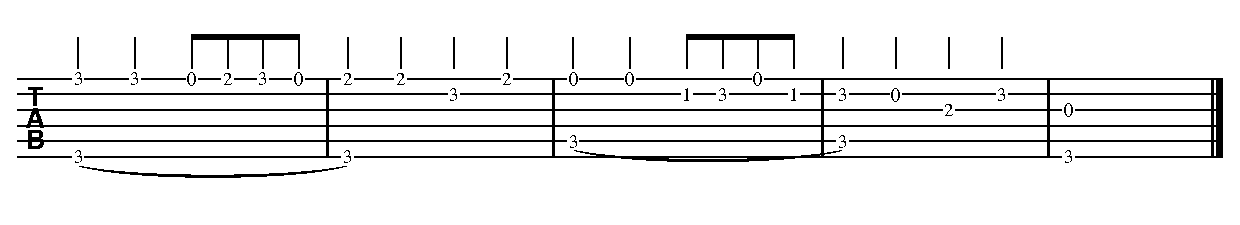
\includegraphics[scale=0.83]{../taby/pohadka.pdf}
% \hspace*{-1.5cm}
\end{centerjustified}

\newpage
\centering
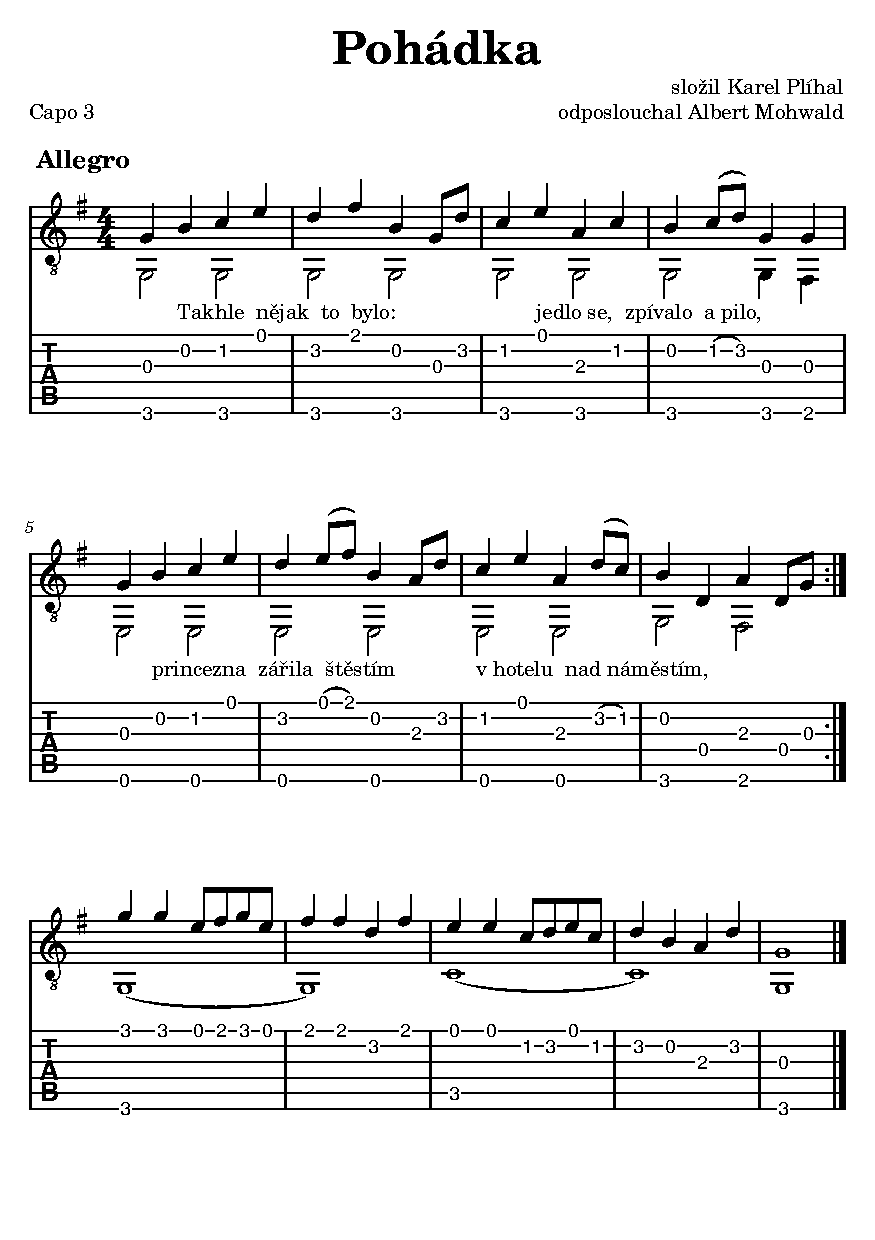
\includegraphics[scale=1.1]{../taby/pohadka-komplet.pdf}

\setcounter{Slokočet}{0}
\end{song}
